\chapter{A model incorporating the experimental data by Mak et al.}

A $Ca^{2+}$ signalling model derived by \citeA{swedish} is currently the only model that includes the open probability, $P_O$,  as modelled in \eqref{foskett} by \citeA{Mak1998}. As discussed previously, the open probability is the probability of the $IP_3R$ being open at any time. \citeA{swedish} derived two models that differed in the way that the opening and closing of the $IP_3R$ worked. These models are based on the model in \citeA{deyoungkeizer}, and the data for the open probability in \citeA{Mak1998}. Each model by \citeA{swedish} produces $Ca^{2+}$ oscillations with different frequencies and amplitudes.

The motivation for their work was to derive a model, based on previous experimental studies, of $Ca^{2+}$ signalling in renal proximal tubular cells following exposure to ouabain \shortcite{ouabain,ouabain2} and after bacterial infection that may cause a fairly common and severe kidney disease in infants \shortcite{uhlensweden}. The paper aims at modelling the impact of store-operated $Ca^{2+}$ on the intracellular $Ca^{2+}$ oscillations, assuming a large concentration gradient between $Ca^{2+}$ in the ER and the cytosol. A large concentration gradient is generally assumed in models of $Ca^{2+}$ signalling \cite{Berridge}, though for oocytes the depletion of the ER is not an essential driving force for oscillations \cite{Sanders2018, wakai}. As discussed in the previous chapter, the $Ca^{2+}$ signals in oocytes are driven by the open probability of the $IP_3R$ and hence the $IP_3R$ dynamics \cite{Mak1998}. In \citeA{swedish} it is acknowledged that the $IP_3R$ are a key mediator of the $Ca^{2+}$ signals \shortcite{patterson}, but it is assumed the oscillations are mainly driven by depletion of the $Ca^{2+}$ stored in the ER. The model, therefore, depends upon the activation of {store-operated channels} on the plasma membrane, rather than receptor-operated channels on the ER, which allow entry of external $Ca^{2+}$ ions into the cytoplasm \shortcite{putney,parekh,parekh2,Kartik,berridge1995}. As a result, they arrive at a reasonably complex model, with a large number of variables. We study this model below and analyse the way in which the experimental data for $P_O$, see equation \eqref{foskett}, has been used.

The model consists of eight ODEs, with the following eight variables : cytosolic $Ca^{2+}$, $c$, $Ca^{2+}$ in the ER, $c_e$, $Ca^{2+}$ in the extracellular volume, $c_{EC}$, cytosolic $IP_3$, $p$, cytosolic G proteins, $G$, store-operated channels in the plasma membrane, ($SOC$), cytosolic $Ca^{2+}$ influx factor, ($CIF_{cyt}$), and in the ER, ($CIF_{ER}$). The extracellular volume is assumed to be infinite. The model is as follows: 
\begin{align}
    \frac{dc}{dt}&=\frac{S_{ER}}{V_{ER}}\beta (J_{channel}-XJ_{pump})-\frac{S_{PM}}{V_{cyt}}\beta (YJ_{in}-J_{pm})\label{swedishc},\\
    \frac{dc_e}{dt}&=\frac{S_{ER}}{V_{ER}}\beta (-J_{channel}+XJ_{pump})\label{swedisher},\\
    \frac{dc_{EC}}{dt}&=0\text{    {(The extracellular volume is ‘infinite’)}},\label{eqeCE}\\
    \frac{dp}{dt}&=\begin{cases}
    G_{signal}I_{deg}p_{max}-I_{deg}p,  &\text{if $t>t_0$}.\\
    -I_{deg}p,  &\text{otherwise}.\label{swedishp}
  \end{cases}\\
    \frac{dG}{dt}&=k_Gc-I_GG,\label{Gode}\\
    \frac{d(SOC)}{dt}&=\frac{S_{PM}}{V_{cyt}}k_{SOC}CIF_{cyt}-I_{SOC}SOC,\label{SOC}\\
    \frac{d(CIF_{cyt})}{dt}&=\frac{S_{ER}}{V_{ER}}\theta c_ev_{CIF}(CIF_{ER}-CIF_{cyt})-\frac{S_{PM}}{V_{cyt}}k_{SOC}CIF_{cyt},\label{cytoCIF}\\
    \frac{d(CIF_{ER})}{dt}&=-\frac{S_{ER}}{V_{ER}r_{ER}}\theta c_ev_{CIF}.\label{ERCIF}
\end{align}
The $Ca^{2+}$ fluxes are given by
\begin{align}
    J_{channel}&=(\textcolor{blue}{V_{IP_3R}}+V_{leak ER})(c_e-c),\label{swedishvip3r}\\
    J_{pump}&=\frac{V_ec}{K_e+c},\nonumber\\
    J_{in}&=\frac{V_pc^2}{K_p^2+c^2},\nonumber\\
    J_{pm}&=(V_{SOC}+V_{leak PM})(c_{EC}-c),\nonumber\\
   G_{signal}&=1-\frac{G^n}{G^n+K_{1/2,G}^n},\nonumber\\
   V_{SOC}&=v_{SOC}SOC,\nonumber\\
   \theta&=\begin{cases}
    1,  &\text{if $c_e<c_{e,min}$}.\nonumber\\
    0,  &\text{otherwise}.\nonumber
  \end{cases}
\end{align}
The biological representations and values of each parameter is given in Table \ref{swedishparam}. Flux through the $IP_3R$ is represented by $J_{channel}$. Flux across the cell plasma membrane is represented by $J_{in}$, and is dependent on the CIF and the SOC channel activity. The two different functions for the $V_{IP_3R}$ term (coloured in blue in equation \eqref{swedishvip3r}) are presented in equations \eqref{vip3r1} and \eqref{vip3r2}. They are based on the $IP_3R$ dynamics in the De Young-Keizer model and on the \citeA{Mak1998} equation for $P_O$ (equation \eqref{foskett}), respectively. For \textcolor{blue}{$V_{IP_3R}$} they choose either
\begin{align}
    V_{IP_3R_1}&=v_1\left(\frac{cpd_2}{(cp+pd_2+d_1d_2+cd_3)(c+d_5)}\right),\label{vip3r1}
\end{align}
or
\begin{align}
    V_{IP_3R_2}&=v_{IP_3R}P_O.\label{vip3r2}
\end{align}
We have equations for cytosolic $Ca^{2+}$ and $Ca^{2+}$ in the ER given by \eqref{swedishc} and \eqref{swedisher} respectively.

The first model in \citeA{swedish} uses equation \eqref{vip3r1}, which was also used in \shortciteA{bakeretal}. This is not specific to any subtype of $IP_3R$. The second model uses equation \eqref{vip3r2} with $P_O$, as derived by \citeA{Mak1998}. We examine how this was implemented and if it fits with the biological representation intended. $V_{IP_3R}$ vs. ${IP_3}$ and $[Ca^{2+}]$, for equations \eqref{vip3r1} and \eqref{vip3r2} respectively, are compared in Figures \ref{deyoungkeizer3d}\textbf{A} and \textbf{B}. The graphs show how the fluxes $V_{IP_3R_1}$ and ${V_IP_3R_2}=v_{IP_3R}P_O$ depend on the $IP_3$ and $Ca^{2+}$ concentrations, respectively. The graphs are quite different. In Figure \ref{deyoungkeizer3d}\textbf{B} we can see that the $IP_3$ concentration saturates at around $0.03\mu M$. When $[IP_3]>0.3 \mu M$, the behaviour of $V_{IP_3R_2}$ does not change significantly as $[Ca^{2+}]$ changes. This is in contrast to Figure \ref{deyoungkeizer3d}\textbf{A} where there is a strong $IP_3$ dependence and the flux is inhibited by very high levels of $Ca^{2+}$. {As $[IP_3]$ increases beyond $0.1\mu M$, the maximum point in the graph in Figure \ref{deyoungkeizer3d}\textbf{A} would continue to grow in a linear manner. However, as we can see in Figure \ref{deyoungkeizer3d}\textbf{B}, the bell-shaped curve has reached a plataeu upon increasing levels of $[IP_3]$.} Although the first model presented in \citeA{swedish} used the $IP_3R$ dynamics from the De Young-Keizer model \eqref{vip3r1}, these were implemented in a different way, as the \citeA{deyoungkeizer} model is not a gating model. Both models in \citeA{swedish} included the open probabilities (from equations \eqref{vip3r1} and \eqref{vip3r2}) in $J_{channel}$.

\begin{figure}[!htb]
\minipage{0.5\textwidth}
  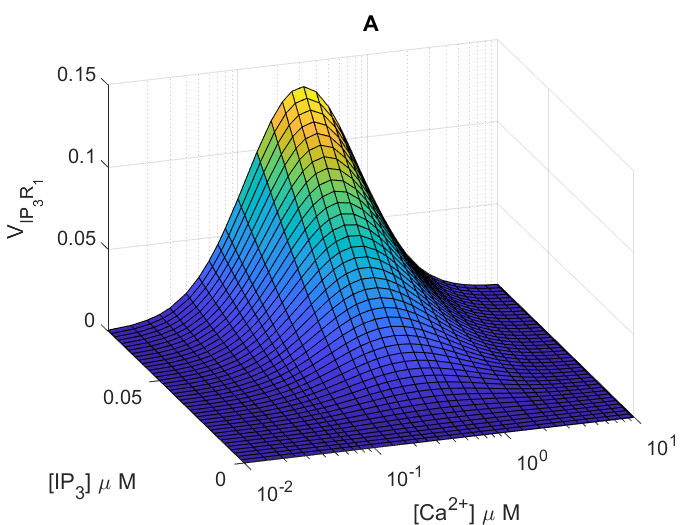
\includegraphics[width=\linewidth]{Chapters/4_Kowalewski_model/extras/deyoungkeizer3d2.png}
\endminipage\hfill
\minipage{0.5\textwidth}
  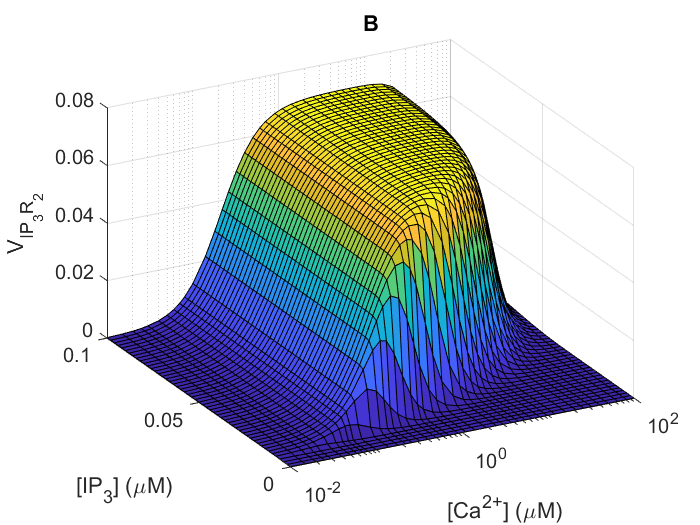
\includegraphics[width=\linewidth]{Chapters/4_Kowalewski_model/extras/swedishmak.png}
\endminipage\hfill
\caption{(\textbf{A}) $V_{IP_3R_1}$ vs. $[IP_3]$ and $[Ca^{2+}]$ ($\mu M$). (\textbf{B}) $V_{IP_3R_2}$ vs. $[IP_3]$ and $[Ca^{2+}]$ ($\mu M$). \cite{swedish,deyoungkeizer, Mak1998} \textit{Software:} MATLAB. }\label{deyoungkeizer3d}
\end{figure}

The two models by \citeA{swedish} exhibit different oscillatory responses for $Ca^{2+}$, as seen in Figure \ref{swedishfig}. With equation \eqref{vip3r1}, $Ca^{2+}$ oscillations with a higher frequency and lower amplitude are generated. A fundamental difference is that the model with equation \eqref{vip3r2} has $Ca^{2+}$ oscillating for all $IP_3$ concentrations higher than $0.012 \mu M$, whereas with equation \eqref{vip3r1} these oscillations were triggered only between $0.030$ and $0.043 \mu M$ \cite{swedish}. 
\begin{figure}[h!!!t!!!b!!!p]
  \centering
  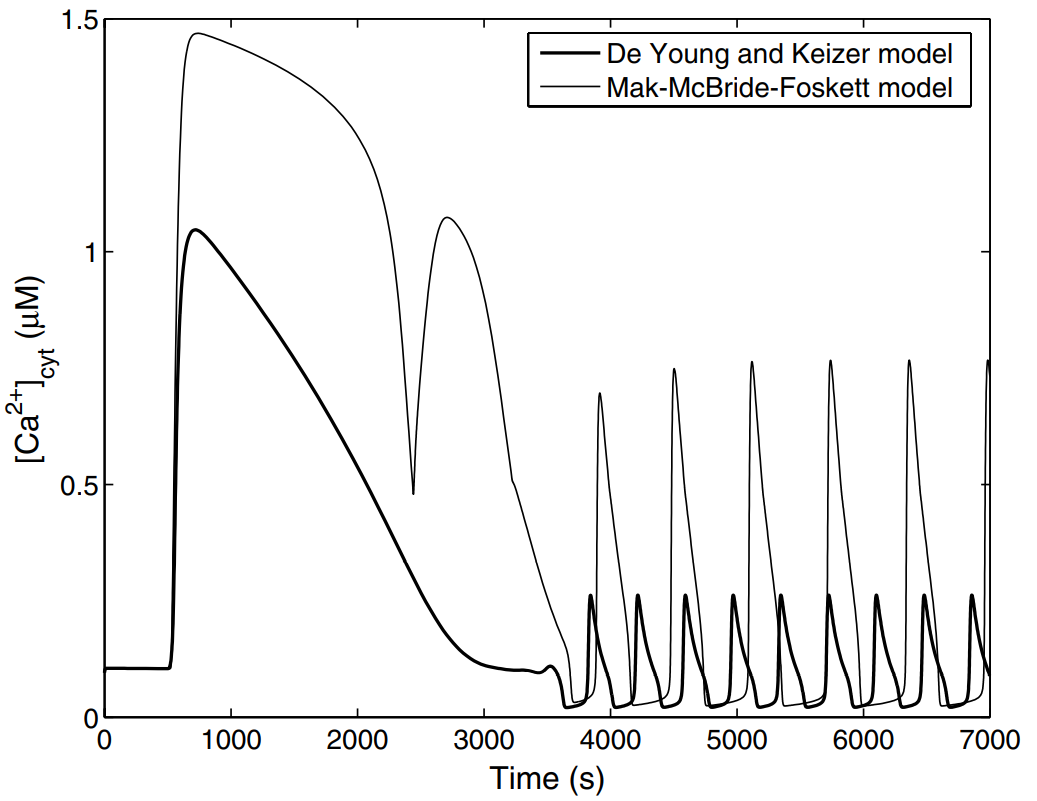
\includegraphics[width=0.8\linewidth]{Chapters/4_Kowalewski_model/extras/swedishfig.png}
  \caption{$Ca^{2+}$ oscillations arising from the two different models by \citeA{swedish}. The `\textit{De Young and Keizer model}' uses equation \eqref{vip3r1} \cite{deyoungkeizer}. The `\textit{Mak-McBride-Foskett model}' uses equation \eqref{vip3r2} \cite{Mak1998}. Source: \citeA{swedish}. {The large difference in their transits is due to the parameters $v_1$ and $v_{IP_3R}$ chosen which represent the maximum $Ca^{2+}$ permeability across the $IP_3R$.} }\label{swedishfig}
\end{figure}

Taking a closer at look the equation for $IP_3$, \eqref{swedishp}, the $IP_3$ concentration starts off at an extremely low level. (See also Table \ref{swedishics}). After a certain amount of time, $t_0=500s$, a reaction is assumed to begin. $IP_3$ has been modelled to degrade linearly with a time constant $1/I_{deg}$. Meanwhile, it is also produced by a reaction controlled by the signal $G_{signal}$. The $G_{signal}$ lies between 0 and 1, and $[IP_3]$ lies between 0 and $IP_{3,max}$. In this model, $[IP_3]$ depends on $G$ (a hypothetical species), that depends on $[Ca^{2+}]$. This is because production of $G$ is proportional to $Ca^{2+}$ and degradation happens at the rate of $I_G[G]$. The parameter $K_{1/2,G}$ is the inactivation constant for the signalling mechanism \cite{swedish}.

A phenomenological model for activating the SOC has been used as the exact mechanism has not yet been identified. The model by \citeA{swedish} has a diffusible messenger and a CIF, and is built upon the idea that CIF exits the ER and binds to a plasma membrane channel. CIF leaves the ER fast and the $Ca^{2+}$ concentration in there decreases. When reaching the plasma membrane, CIF then binds to and activates SOC. The SOC are then deactivated after a while so long as more CIF has not been released into the cytosol. Within the ER CIF is regenerated at a slow pace but only let out when the ER $Ca^{2+}$ level is lower than the threshold of $10 \mu M$ \cite{swedish}.

\begin{table}[h!!!t!!!b!!!p]
\begin{center}
\begin{tabular}{ c c c c c}
Variable & Initial value\\
\hline
Cytosolic $IP_3$ & $1pM$ \\
\hline
ER $Ca^{2+}$ & $100 \mu M$\\
\hline
ER CIF & $0.1 \mu M$\\
\hline
Cytosolic G & $0$\\
\hline
Cytosolic $Ca^{2+}$ & $95 nM$\\
\hline
Extracellular $Ca^{2+}$ & $950 \mu M$\\
\hline
Cytosolic CIF & $0$\\
\hline
Active SOC in plasma membrane & $0$\\
\end{tabular}
\end{center}
\caption{Initial values used for the models in Kowalewski et al \cite{swedish}.}\label{swedishics}
\end{table}

 Both models in \citeA{swedish} generate $Ca^{2+}$ oscillations (see Figure \ref{swedishfig}). However, it is difficult to compare these oscillations to $Ca^{2+}$ oscillations at fertilisation as many other variables (that are not relevant to the cell type we are looking at) are included. The models rely on the existence of SOC, for example. One explanation for the activation of SOC is the assumed depletion of $Ca^{2+}$ from the ER. As previously discussed, a model where $Ca^{2+}$ released from the ER is a driving force for oscillations is not appropriate for $Ca^{2+}$ signalling in fertilisation. Experimental data in \citeA{Sanders2018, wakai} {suggest} that cytosolic $Ca^{2+}$ oscillations in an egg rely on the $IP_3R$ dynamics to be the main driving force, and that ER store depletion plays a much less significant role. The model by \citeA{swedish} is therefore not appropriate for the mammalian egg. We must derive a new model that is appropriate incorporating the data from \citeA{Mak1998}.

We hence face the challenge of  appropriately incorporating the open probability from equation \eqref{foskett} into a new model that does not strongly depend on depletion of $Ca^{2+}$ from the ER. We will use the knowledge acquired from this chapter and our literature review to derive a new such model in Chapter 5. 
